%%\documentclass[a4paper,12pt,oneside]{llncs}
\documentclass[12pt,letterpaper]{article}
\usepackage[right=2cm,left=3cm,top=2cm,bottom=2cm,headsep=0cm]{geometry}

%%%%%%%%%%%%%%%%%%%%%%%%%%%%%%%%%%%%%%%%%%%%%%%%%%%%%%%%%%%
%% Juego de caracteres usado en el archivo fuente: UTF-8
\usepackage{ucs}
\usepackage[utf8x]{inputenc}

%%%%%%%%%%%%%%%%%%%%%%%%%%%%%%%%%%%%%%%%%%%%%%%%%%%%%%%%%%%
%% Juego de caracteres usado en la salida dvi
%% Otra posibilidad: \usepackage{t1enc}
\usepackage[T1]{fontenc}

%%%%%%%%%%%%%%%%%%%%%%%%%%%%%%%%%%%%%%%%%%%%%%%%%%%%%%%%%%%
%% Ajusta maergenes para a4
%\usepackage{a4wide}

%%%%%%%%%%%%%%%%%%%%%%%%%%%%%%%%%%%%%%%%%%%%%%%%%%%%%%%%%%%
%% Uso fuente postscript times, para que los ps y pdf queden y pequeños...
\usepackage{times}

%%%%%%%%%%%%%%%%%%%%%%%%%%%%%%%%%%%%%%%%%%%%%%%%%%%%%%%%%%%
%% Posibilidad de hipertexto (especialmente en pdf)
%\usepackage{hyperref}
\usepackage[bookmarks = true, colorlinks=true, linkcolor = black, citecolor = black, menucolor = black, urlcolor = black]{hyperref}

%%%%%%%%%%%%%%%%%%%%%%%%%%%%%%%%%%%%%%%%%%%%%%%%%%%%%%%%%%%
%% Graficos 
\usepackage{graphics,graphicx}

%%%%%%%%%%%%%%%%%%%%%%%%%%%%%%%%%%%%%%%%%%%%%%%%%%%%%%%%%%%
%% Ciertos caracteres "raros"...
\usepackage{latexsym}

%%%%%%%%%%%%%%%%%%%%%%%%%%%%%%%%%%%%%%%%%%%%%%%%%%%%%%%%%%%
%% Matematicas aun más fuertes (american math dociety)
\usepackage{amsmath}

%%%%%%%%%%%%%%%%%%%%%%%%%%%%%%%%%%%%%%%%%%%%%%%%%%%%%%%%%%%
\usepackage{multirow} % para las tablas
\usepackage[spanish,es-tabla]{babel}

%%%%%%%%%%%%%%%%%%%%%%%%%%%%%%%%%%%%%%%%%%%%%%%%%%%%%%%%%%%
%% Fuentes matematicas lo mas compatibles posibles con postscript (times)
%% (Esto no funciona para todos los simbolos pero reduce mucho el tamaño del
%% pdf si hay muchas matamaticas....
%\usepackage{mathptm}

%%% VARIOS:
%\usepackage{slashbox}
\usepackage{verbatim}
\usepackage{array}
\usepackage{listings}
\usepackage{multirow}

%% MARCA DE AGUA
%% Este package de "draft copy" NO funciona con pdflatex
%%\usepackage{draftcopy}
%% Este package de "draft copy" SI funciona con pdflatex
%%%\usepackage{pdfdraftcopy}
%%%%%%%%%%%%%%%%%%%%%%%%%%%%%%%%%%%%%%%%%%%%%%%%%%%%%%%%%%%
%% Indenteacion en español...
\usepackage[spanish]{babel}
\usepackage[svgnames,x11names,table]{xcolor}
\usepackage{listings}
% Para escribir código en C
% \begin{lstlisting}[language=C]
% #include <stdio.h>
% int main(int argc, char* argv[]) {
% puts("Hola mundo!");
% }
% \end{lstlisting}


\title{Apache Flink}
\author{Jesús Rodríguez Heras\\Roberto Muras González\\Juan Pedro Rodríguez Gracia\\Gabriel Fernando Sánchez Reina}

\begin{document}
	
	\maketitle
	\begin{abstract} %Poner esto en todas las prácticas de PCTR
		\begin{center}
			Definición de Apache Flink y ejemplo de uso capturando datos de una red social con RabbitMQ como broker de mensajería.
		\end{center}
	\end{abstract}
	\thispagestyle{empty}
	\newpage
	
	\tableofcontents
	\newpage
	
	%%\listoftables
	%%\newpage
	
	%%\listoffigures
	%%\newpage
	
	%%%% REAL WORK BEGINS HERE:
	
	%%Configuracion del paquete listings
	\lstset{language=bash, numbers=left, numberstyle=\tiny, numbersep=10pt, firstnumber=1, stepnumber=1, basicstyle=\small\ttfamily, tabsize=1, extendedchars=true, inputencoding=latin1}


\section{Introducción}
\subsection{¿Qué es Apache Flink?}
Se trata de un motor de procesamiento de streams o flujos de datos de código abierto que proporciona capacidades de distribución de datos, comunicaciones y, muy importante, tolerancia a fallos a las computaciones.\\

El núcleo de Apache Flink es un motor de flujo de datos de transmisión distribuida escrito en Java y Scala. El sistema de tiempo de ejecución encadenado de Flink, permite la ejecución de programas de procesamiento por bloques y de flujo.

\subsection{¿Qué es RabbitMQ?}
Es un software de negociación de mensajes de código abierto. Se encuentra dentro de la categoría de middleware de mensajería. Implementa el estándar ``Advanced Message Queuing Protocol'' (AMQP).\\

El servidor de RabbitMQ está escrito en Erlang y utiliza el framework ``Open Telecom Platform'' (OTP) para construir sus capacidades de ejecución distribuida y conmutación ante errores.


\section{Guía de instalación}
\subsection{Instalación de Java}
Lo primero que necesitaremos para instalar Apache Flink, será tener java instalado. Para ello, nos movemos a la carpeta en la que queramos instalarlo en nuestro caso será \texttt{/usr/java}, en caso de no tener esta carpeta haremos \texttt{mkdir java} para ello abrimos una terminal en el directorio raíz y ejecutamos la siguiente orden: \texttt{cd /usr/java}.
\begin{center}
	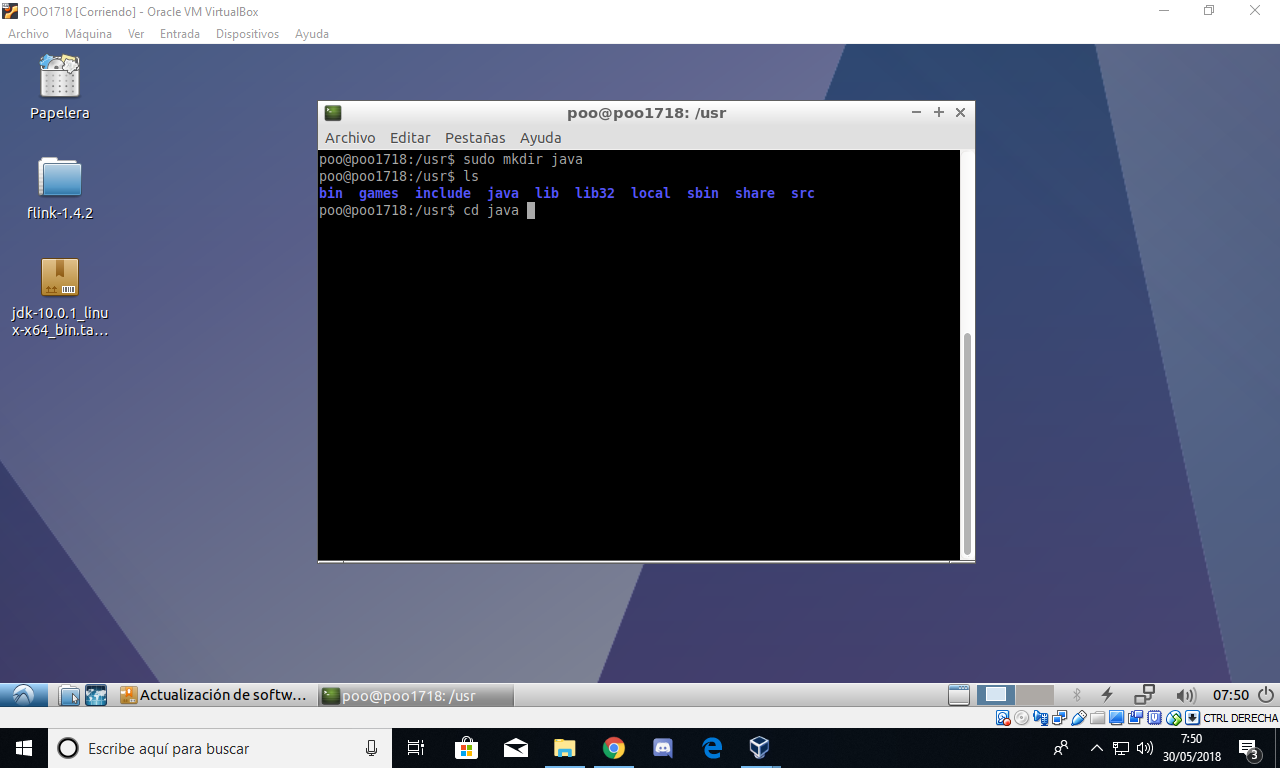
\includegraphics[scale=0.5]{1.png}\\
	
	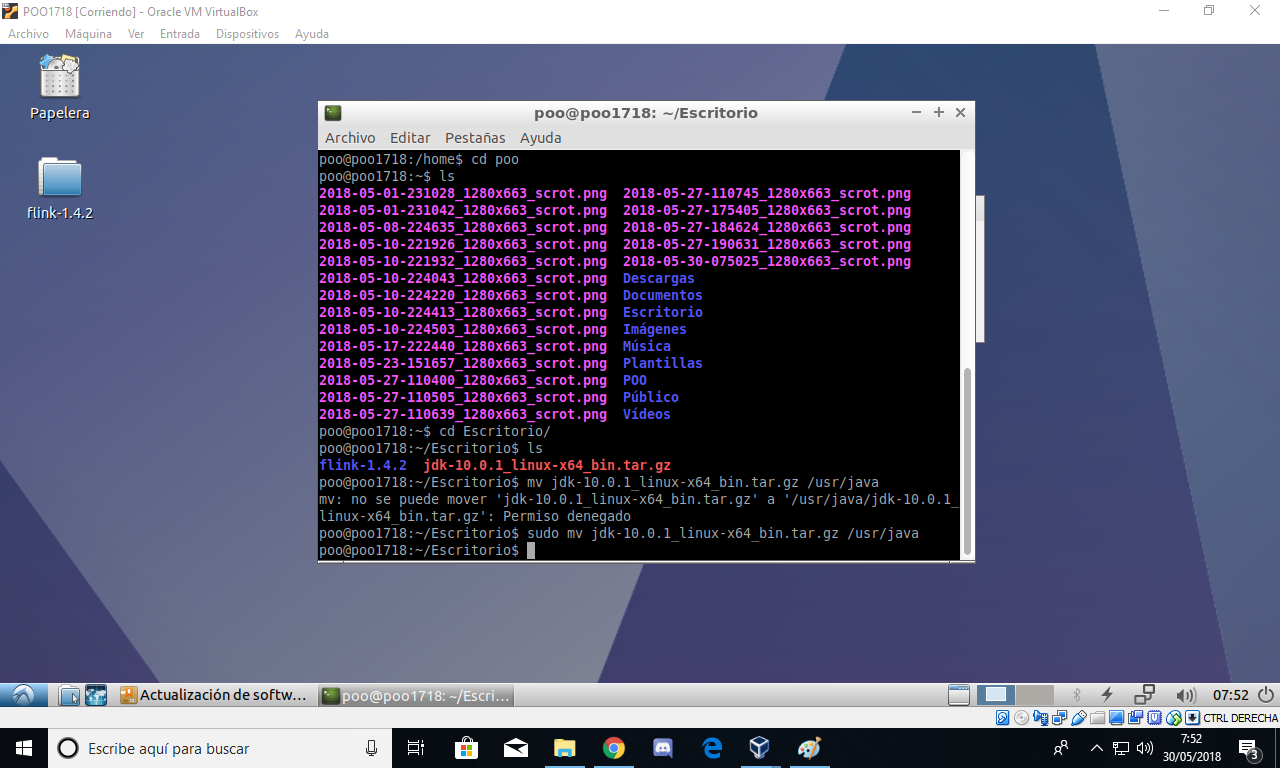
\includegraphics[scale=0.5]{2.png}
\end{center}
Ahora nos descargamos java de la página principal de java. \url{https://www.java.com/es/download/help/linux_x64_install.xml} 
El paso siguiente será mover el comprimido a dicha raíz, para ello, ejecutamos la siguiente orden, \texttt{mv NombreDescarga /usr/java}.
\begin{center}
	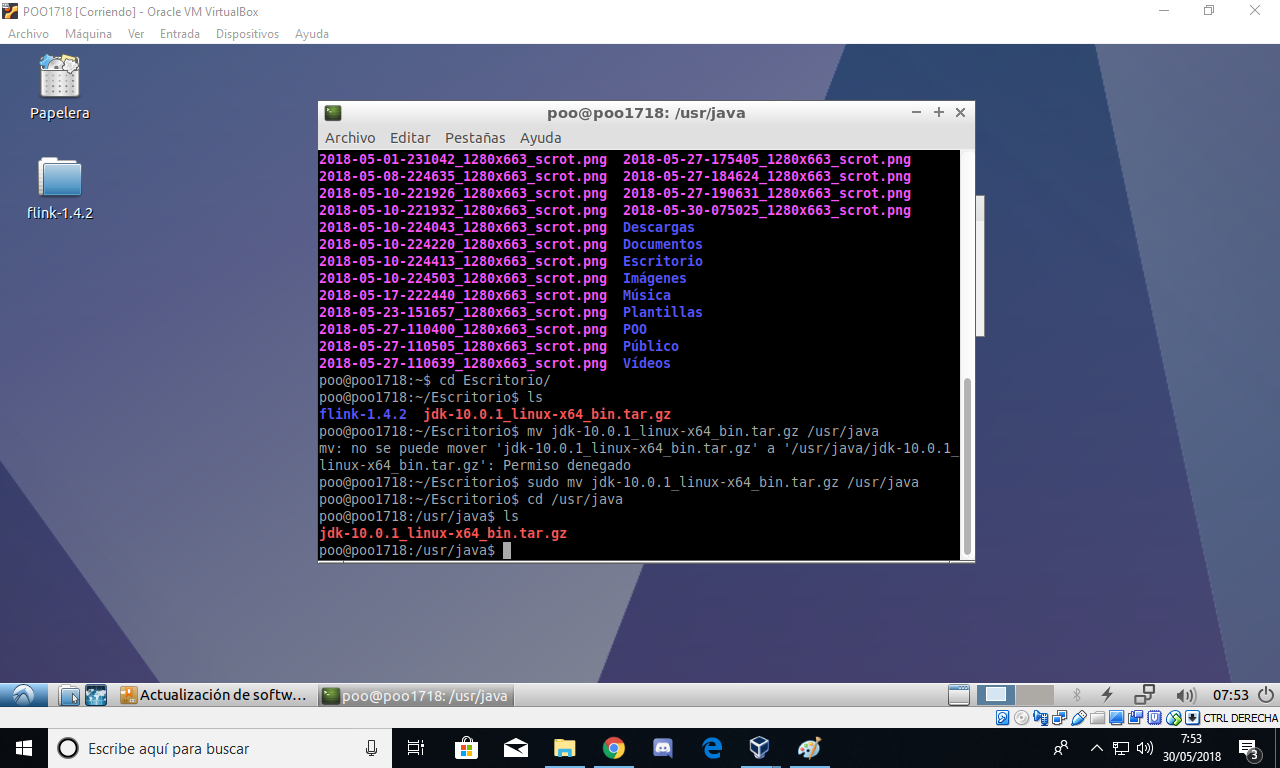
\includegraphics[scale=0.5]{3.png}
\end{center}
Tras esto, ejecutamos el siguiente comando para descomprimir e instalar el archivo previamente descargado, \texttt{tar zxvf NombreDescarga}.
\begin{center}
	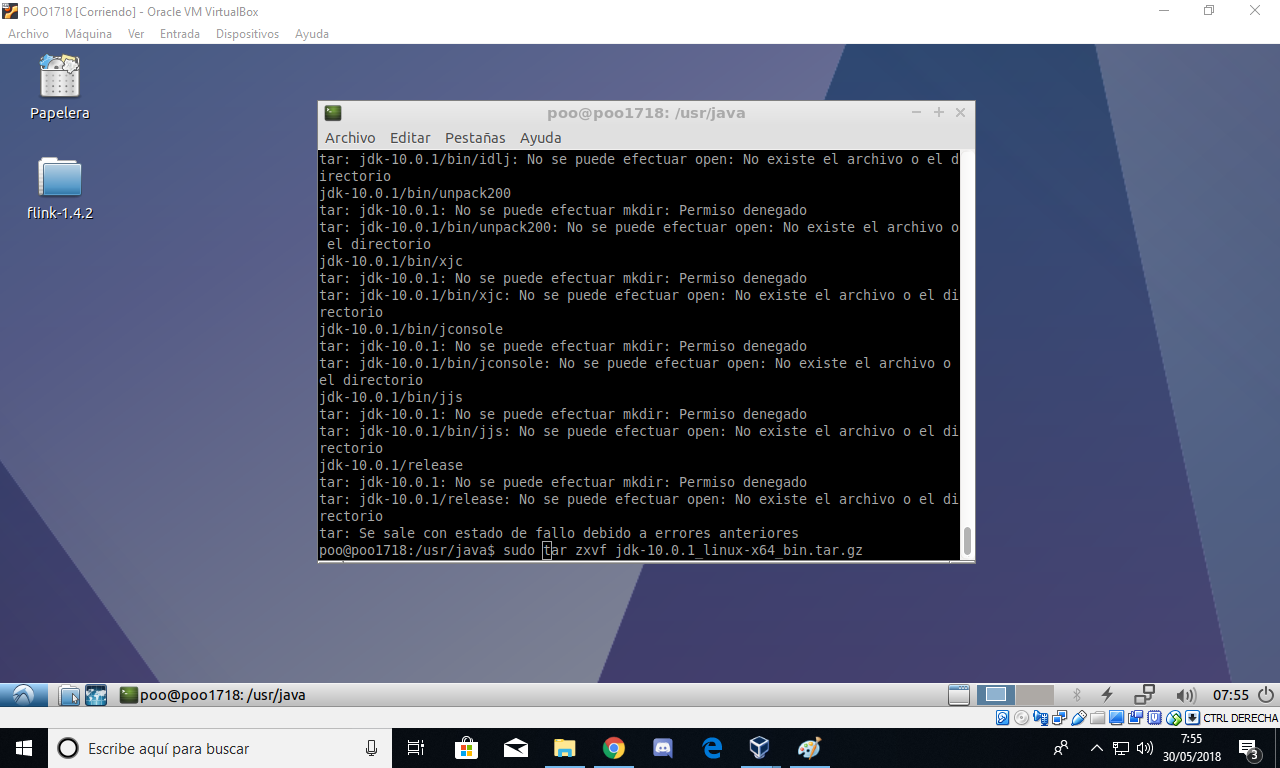
\includegraphics[scale=0.5]{4.png}
\end{center}
Con esto, tendríamos ya instalado java. Ahora tendríamos que asignar la variable \texttt{JAVA\_HOME}, para ello, ejecutamos el siguiente comando: \texttt{export JAVA\_HOME=/usr/java/VersiónInstalada}. Para comprobar que está bien ejecutado, haremos \texttt{echo \$JAVA\_HOME}.
\begin{center}
	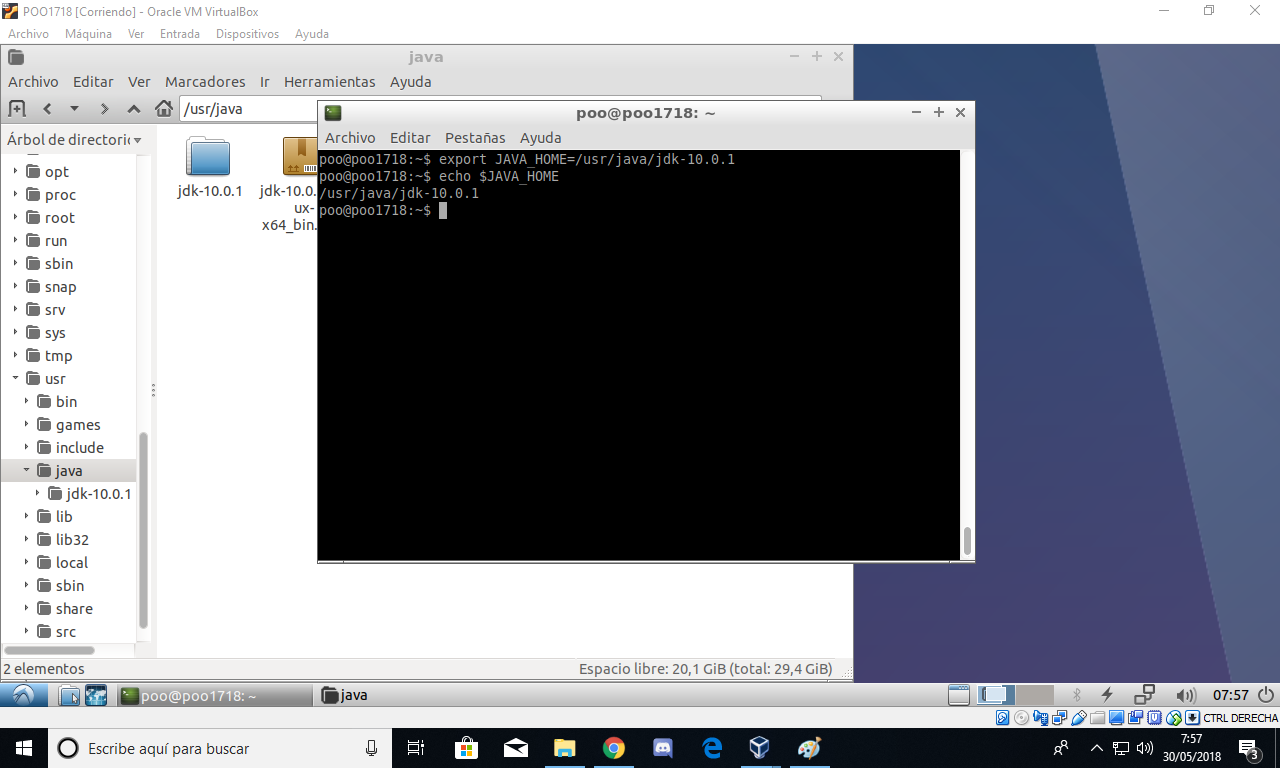
\includegraphics[scale=0.5]{5.png}
\end{center}

\subsection{Apache Flink}
Una vez hecho lo anterior, procedemos a la instalación de Apache Flink, para ello debemos descargarnos Apache Flink de la página principal de Apache: \url{https://flink.apache.org/downloads.html} 
Una vez lo tengamos descargado, lo extraemos en la carpeta que deseemos y accedemos a ella a través de la terminal.\\

Accederemos a la configuración para cambiar el puerto al que se  conecta Apache Flink, para ello hacemos \texttt{cd conf} y allí hacemos un ``\texttt{vi}'' del archivo de configuración (flink-conf.yaml) o directamente abrir este archivo con un editor de texto y hacer los cambios pertinentes.
\begin{center}
	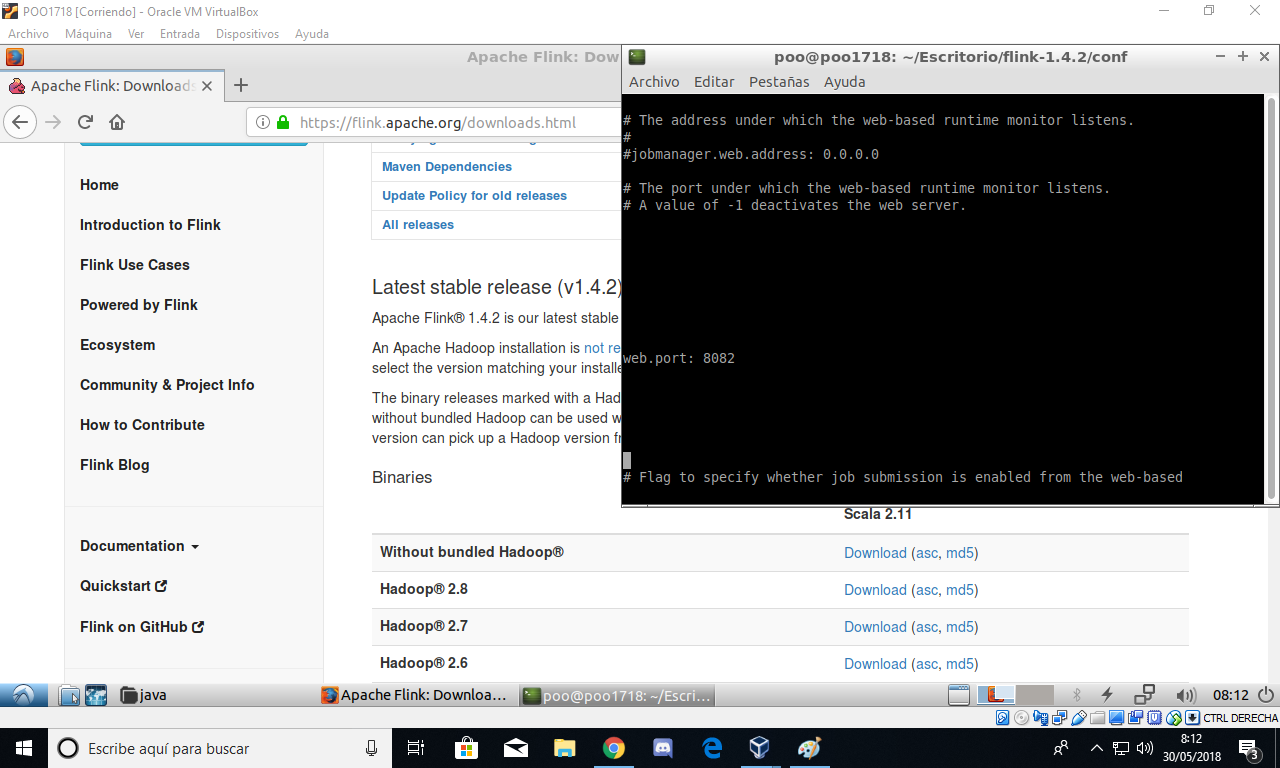
\includegraphics[scale=0.5]{6.png}\\
	
	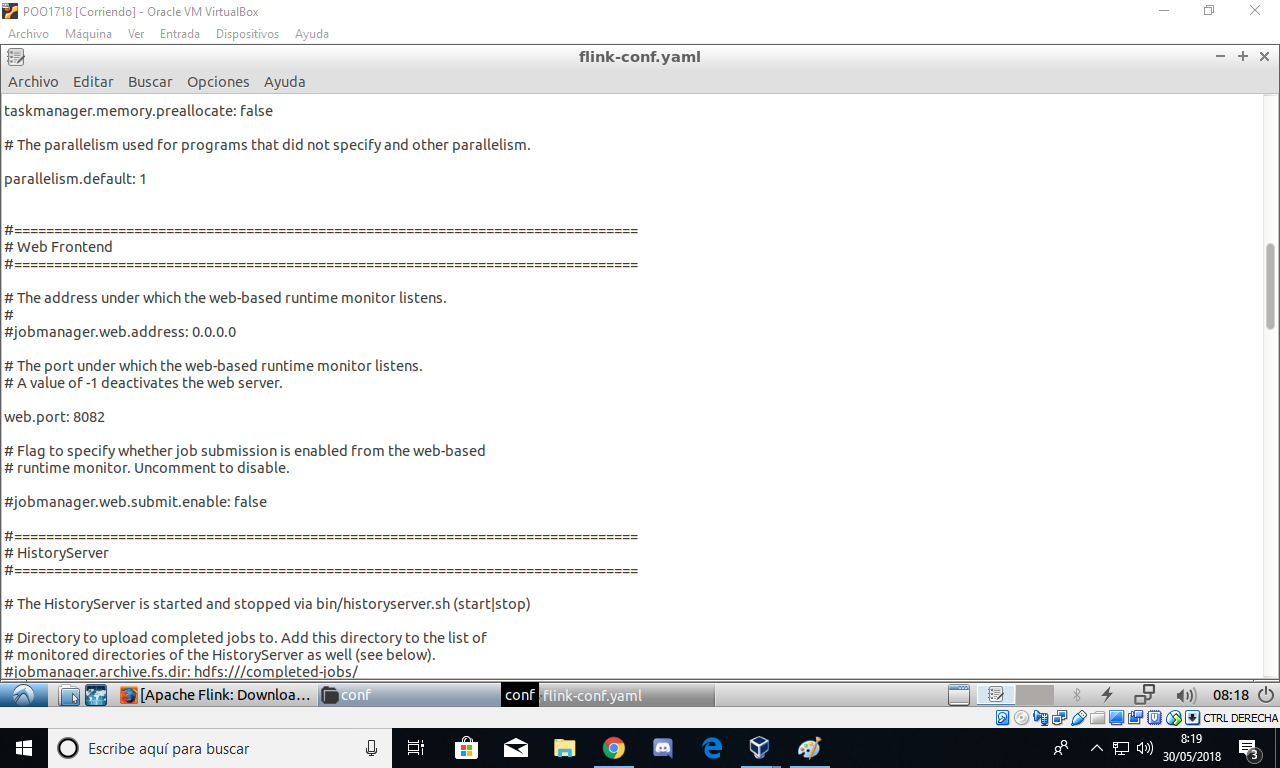
\includegraphics[scale=0.5]{7.png}
\end{center}
Lo siguiente que haremos será ejecutar flink, para ello haremos \texttt{cd bin} y ejecutamos el archivo llamado \texttt{start-cluster.sh}.
\begin{center}
	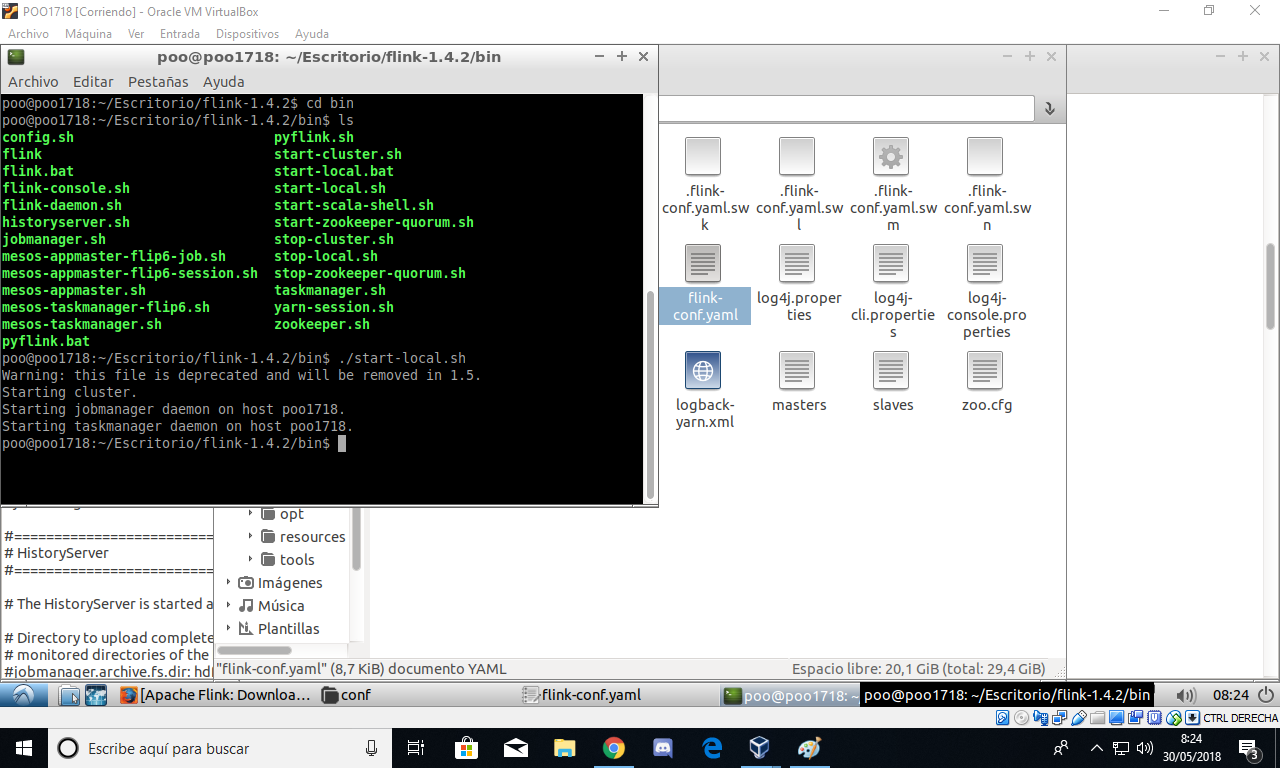
\includegraphics[scale=0.5]{8.png}
\end{center}
Para saber si se ha ejecutado correctamente, entramos en el navegador web y escribimos \url{localhost:PuertoAsignado} y nos mostrará lo siguiente:
\begin{center}
	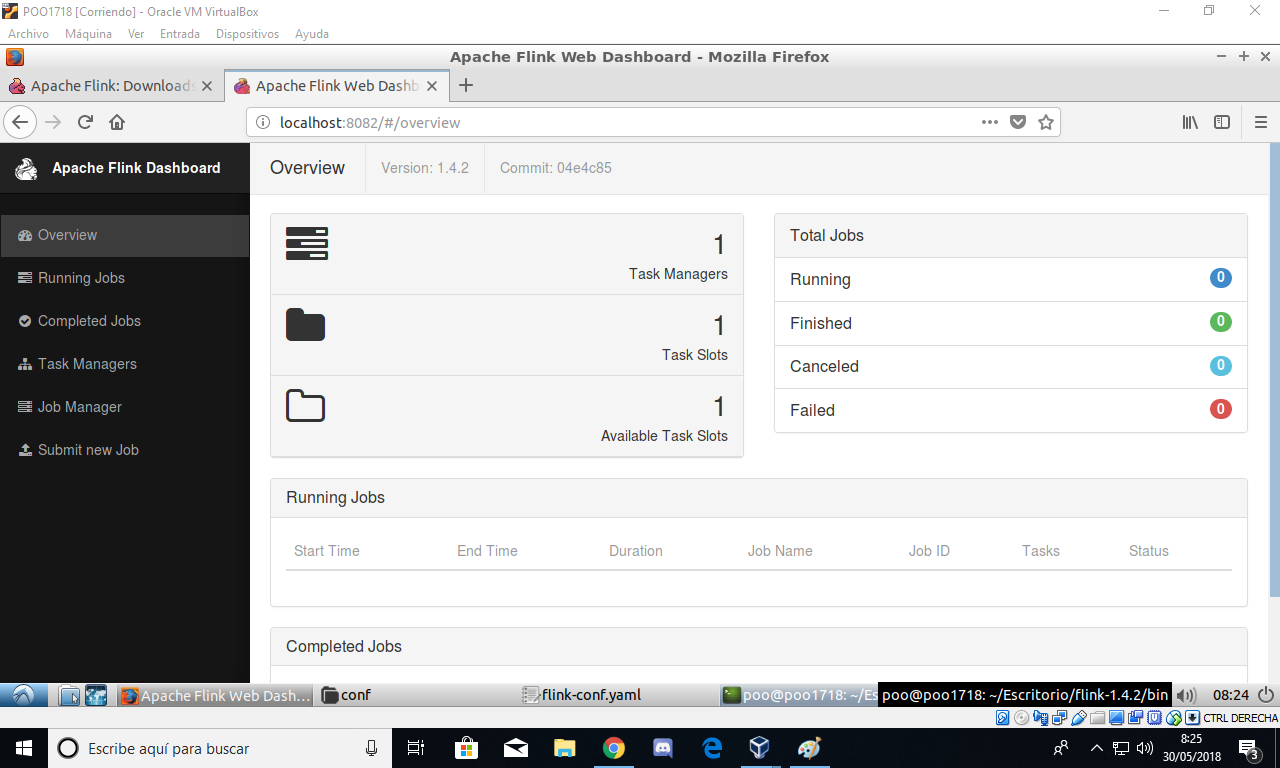
\includegraphics[scale=0.5]{9.png}
\end{center}

\subsubsection{Prueba de Apache Flink}
Pasaremos ahora a ejecutar una prueba. Para ejecutar el programa de prueba tendremos que tener creado el fichero \texttt{input.txt}.
\begin{center}
	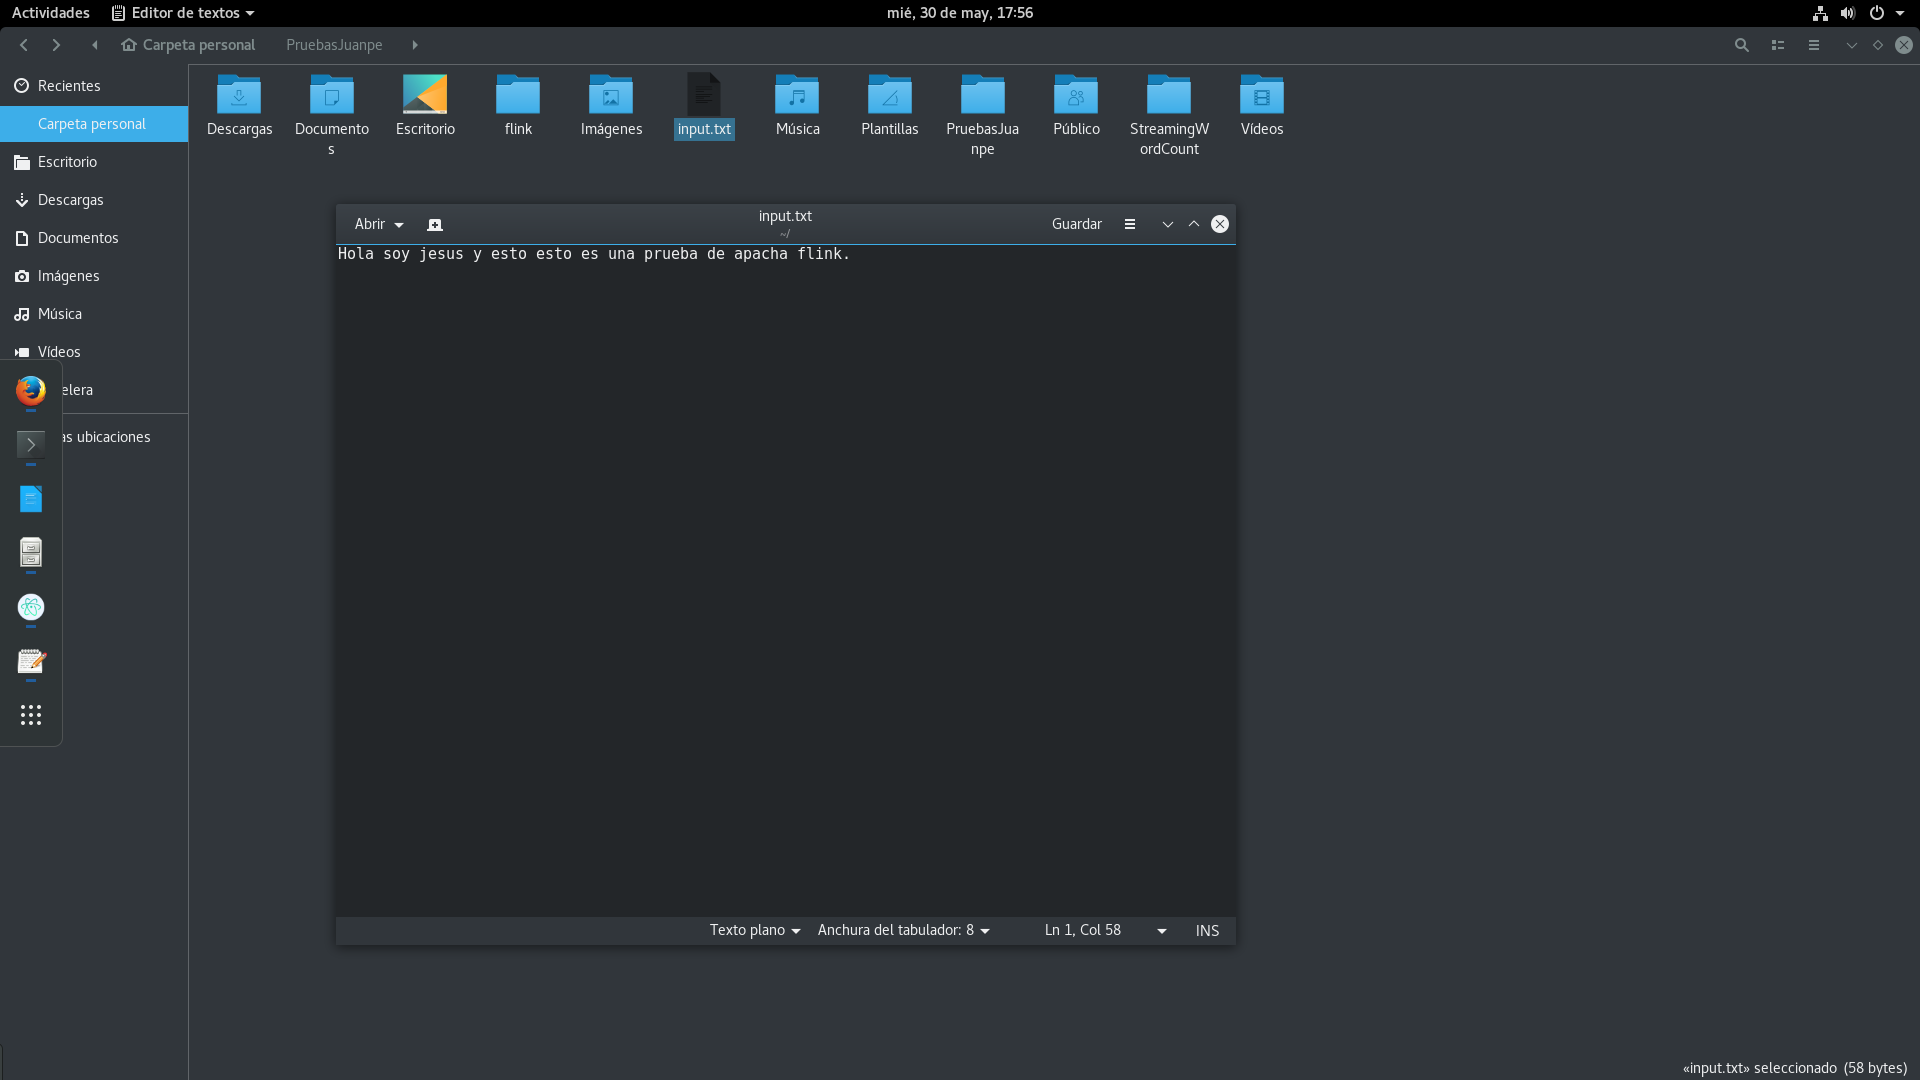
\includegraphics[scale=0.24]{13.png}
	Un detalle sin importancia es la repetición de la palabra ``esto'' y ``apacha'' en lugar de ``apache''.
\end{center}

Ahora, basta con ejecutar el siguiente comando desde la carpeta de flink \texttt{bin/flink run examples/batch/WordCount.jar -input /home/jesus/input.txt -output}\\\texttt{/home/jesus/ouput.txt}.\\

\begin{center}
	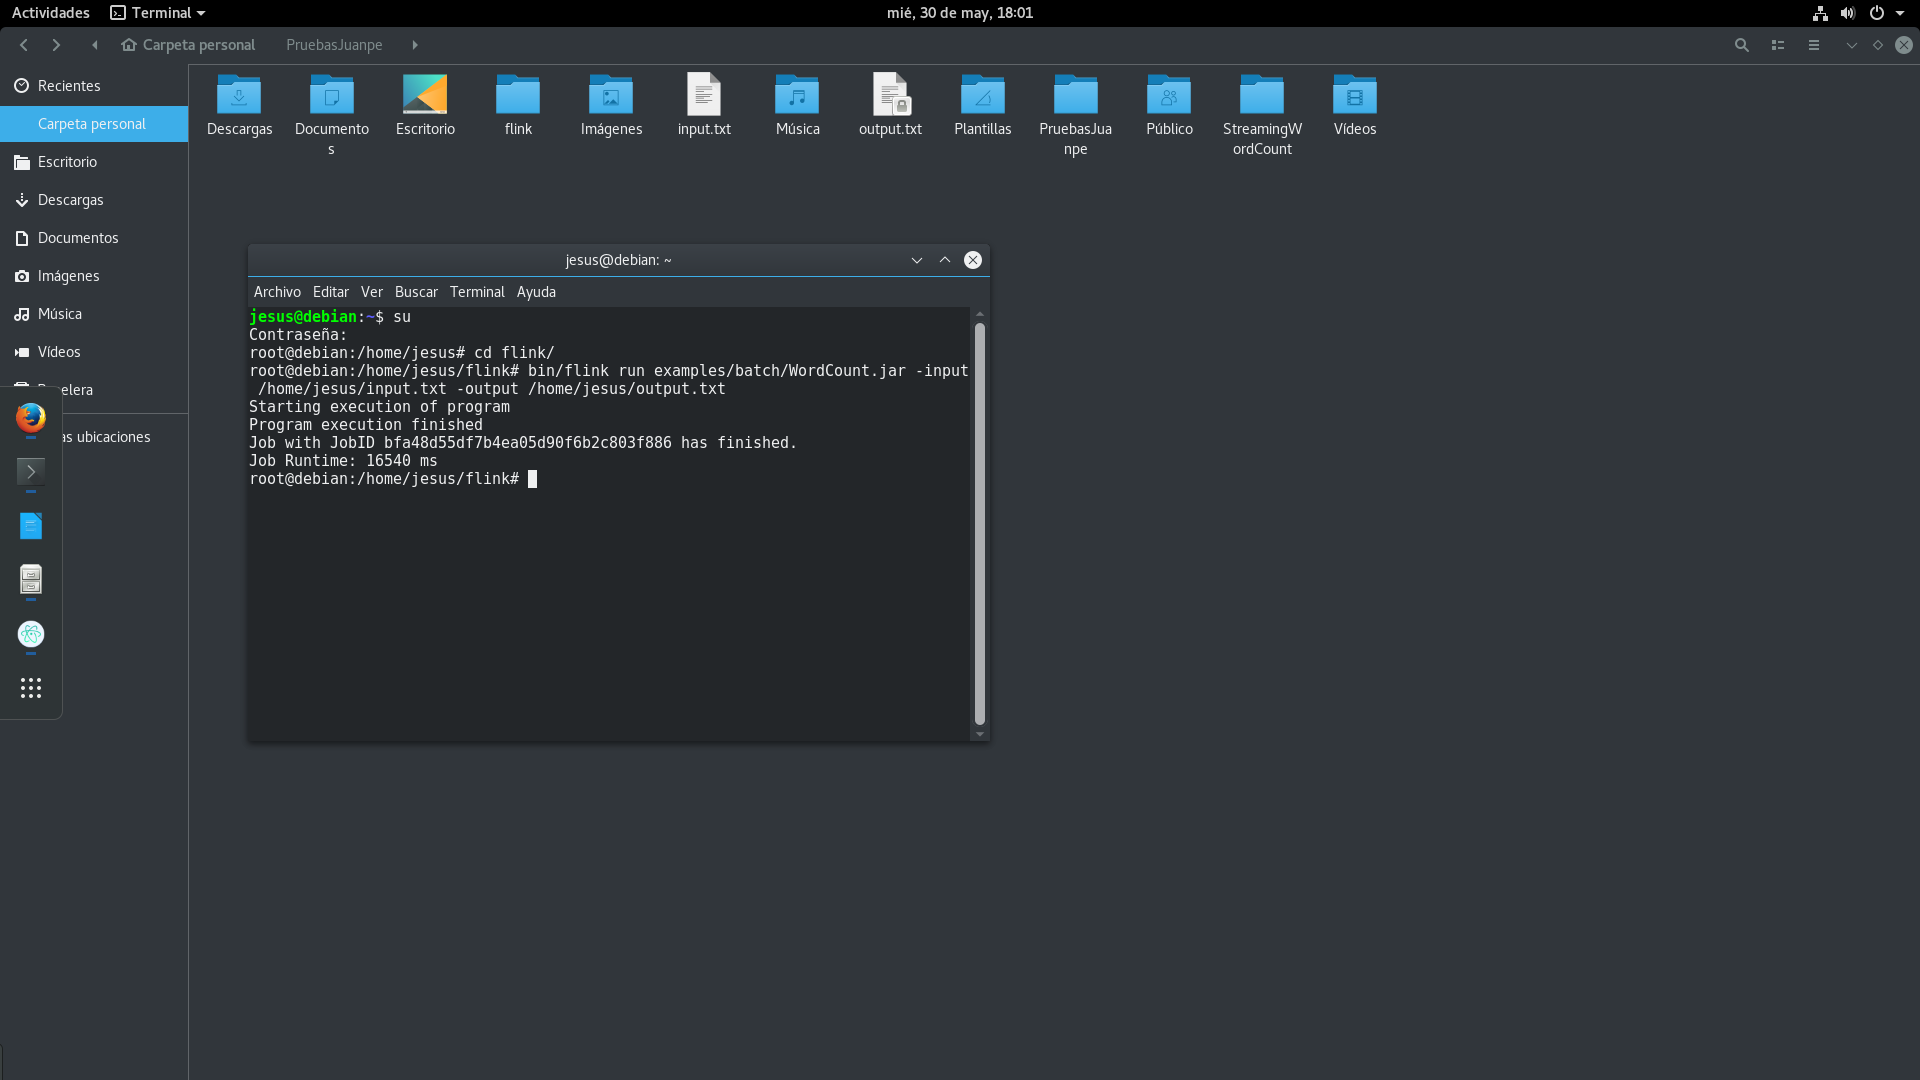
\includegraphics[scale=0.24]{14.png}
\end{center}

Y obtenemos el recuento de palabras en el fichero \texttt{output.txt} que se ha creado con la ejecución del programa.
\begin{center}
	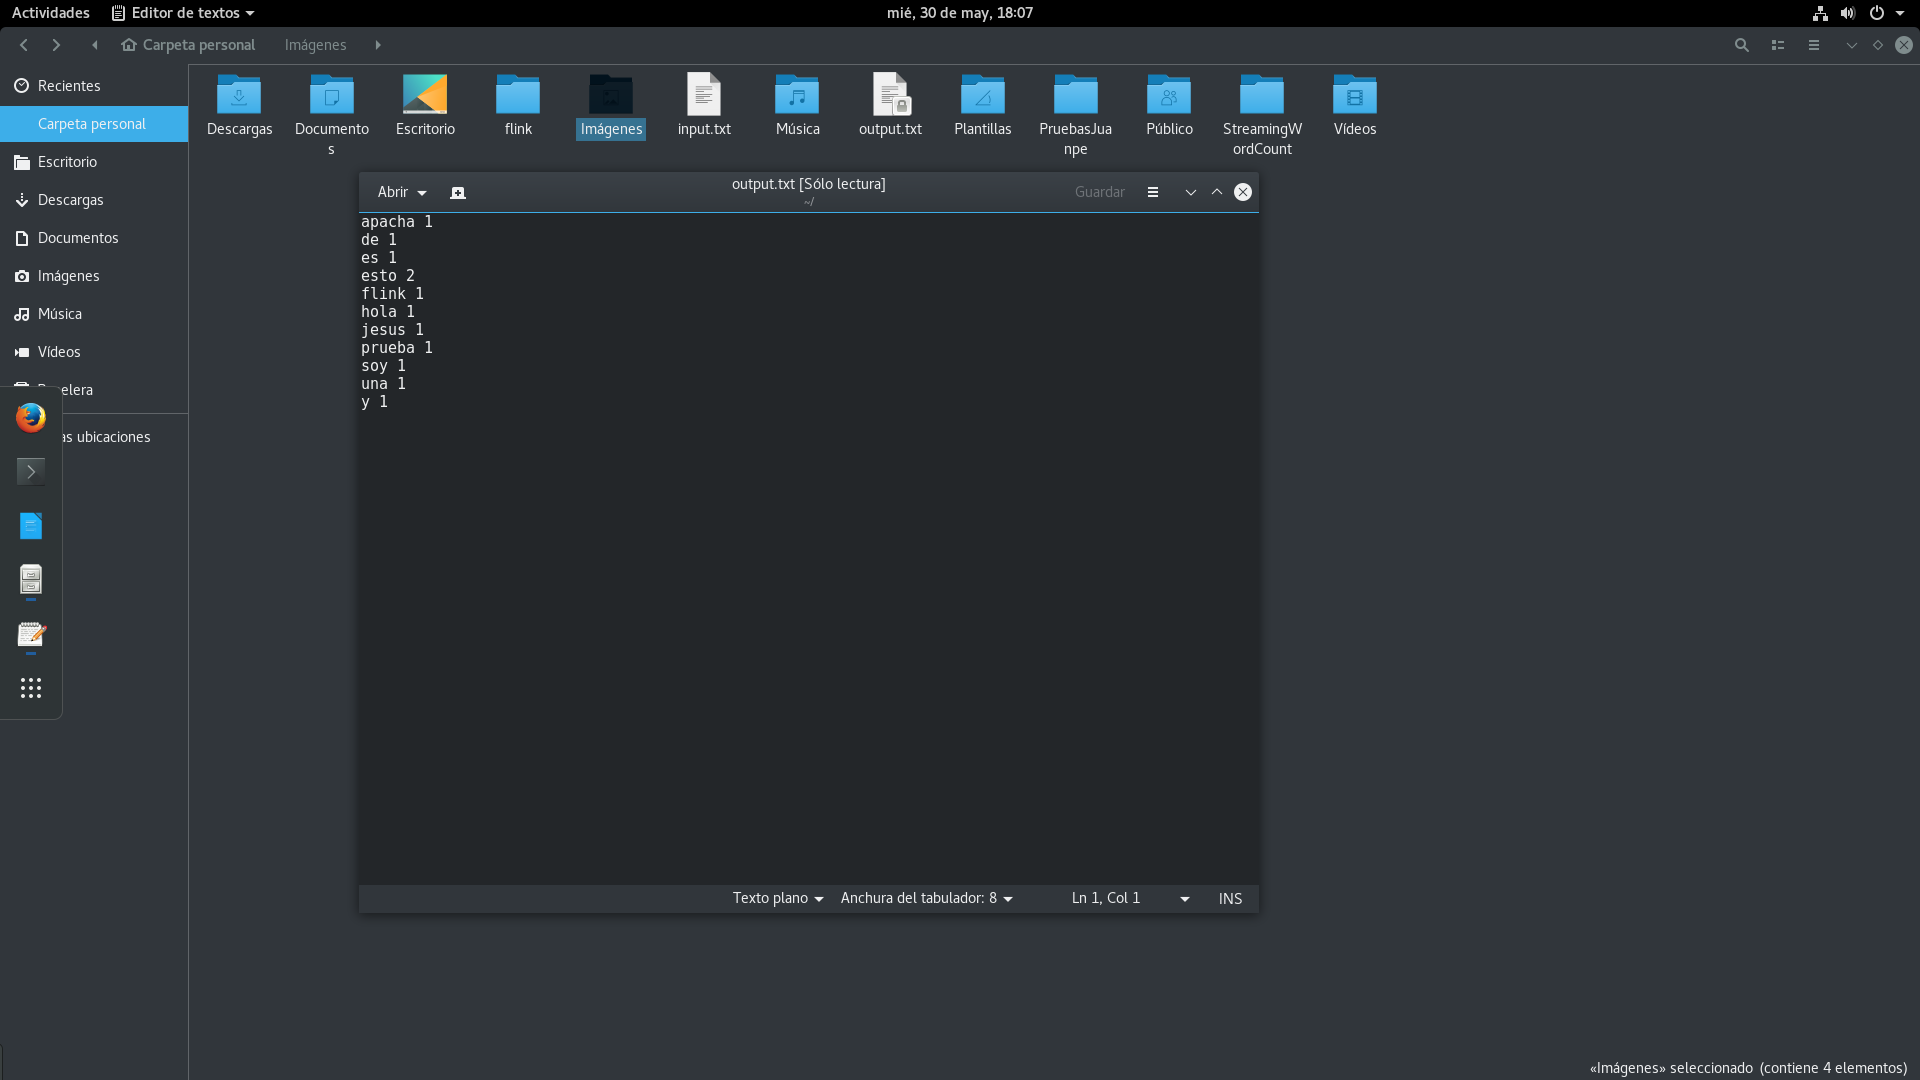
\includegraphics[scale=0.24]{15.png}
\end{center}


\subsection{RabbitMQ}
Para la instalación de RabbitMQ lanzaremos el siguiente comando en la terminal: \texttt{sudo apt-get install rabbitmq-server}.\\

Una vez terminado el proceso, instalaremos la consola de administración con el comando \texttt{sudo rabbitmq-plugins enable rabbitmq\_management}.\\

A continuación, y para ver que funciona, nos dirigimos a la siguiente dirección con nuestro navegador: \url{http://localhost:15672} donde entraremos con el usuario \texttt{guest} y la contraseña \texttt{guest}.

\section{Palabras más publicadas en twitter}
%Implementar algo que use estas dos tecnologías junto con twitter
Nuestro proyecto se centra en contar las palabras más publicadas en twitter por la población española. Cuenta con dos archivos escritos en Python: \texttt{tareas.py} y \texttt{receptor.py} que se encargarán de recolectar los mensajes. Luego, el contador de palabras de prueba de Apache Flink se encargará del resto.\\

Lo primero de todo es iniciar Apache Flink ejecutando el fichero \texttt{start-cluster.sh} ubicado en \texttt{/home/flink/bin/} y ejecutar la consola de administración de RabbitMQ con \texttt{sudo rabbtimq-plugins enable rabbitmq\_management}.\\

Luego ejecutamos el archivo \texttt{tareas.py} que se encarga de entrar en twitter y, de entre todos los Trending Topics españoles actuales, elige el primero, recopila los 100 ultimos tweets asociados a dicho Trending Topic y los envía a la cola de mensajes de RabbitMQ como una sola cadena de texto.\\

A continuación, el archivo \texttt{receptor.py} se encarga de vaciar la cola de mensajes y escribir su contenido en el fichero \texttt{input.txt} ubicado en \texttt{/home/jesus/}.

\begin{center}
	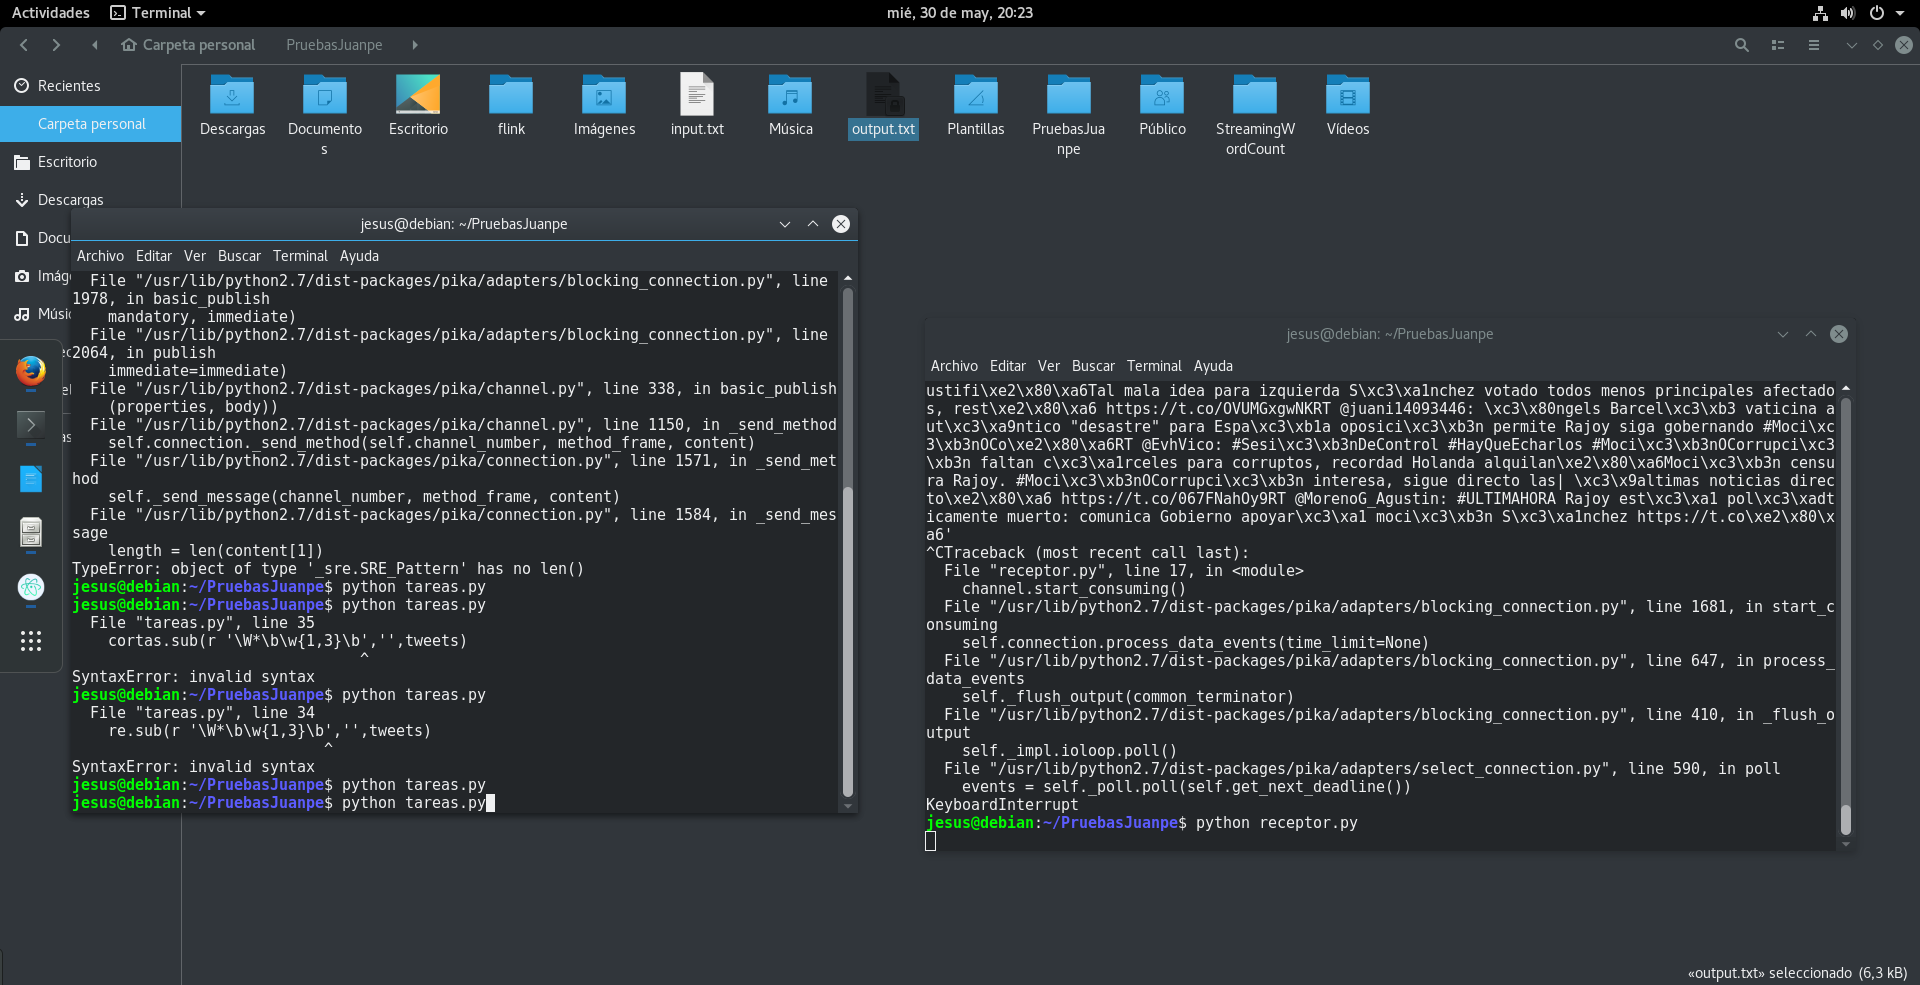
\includegraphics[scale=0.24]{16.png}\\
	
	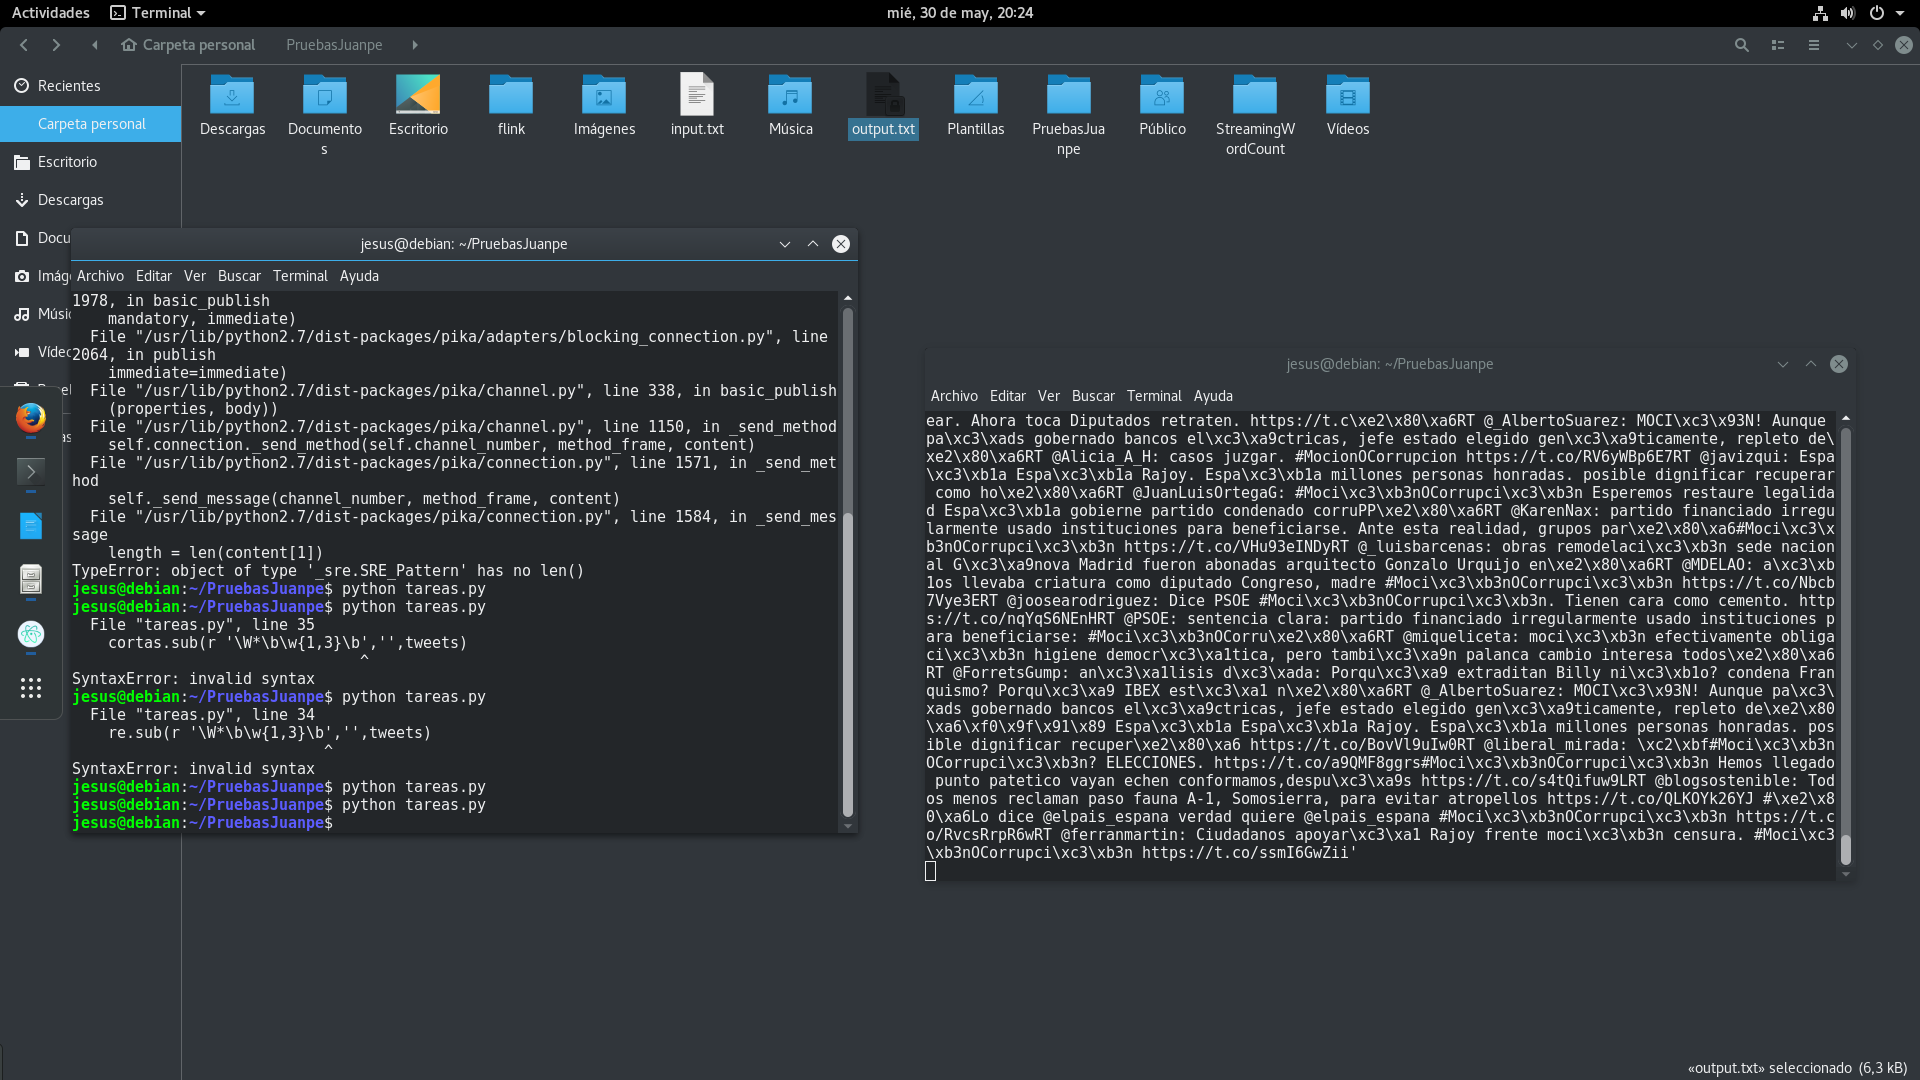
\includegraphics[scale=0.24]{17.png}
\end{center}

Por último, ejecutando el contador de palabras del ejemplo anteriormente comentado en la prueba de Apache Flink, obtenemos el fichero \texttt{output.txt} con el número de repeticiones que tiene cada palabra. Para ello usaremos el comando \texttt{bin/flink run examples/batch/WordCount.jar -input /home/jesus/input.txt -output /home/jesus/output.txt}.
\begin{center}
	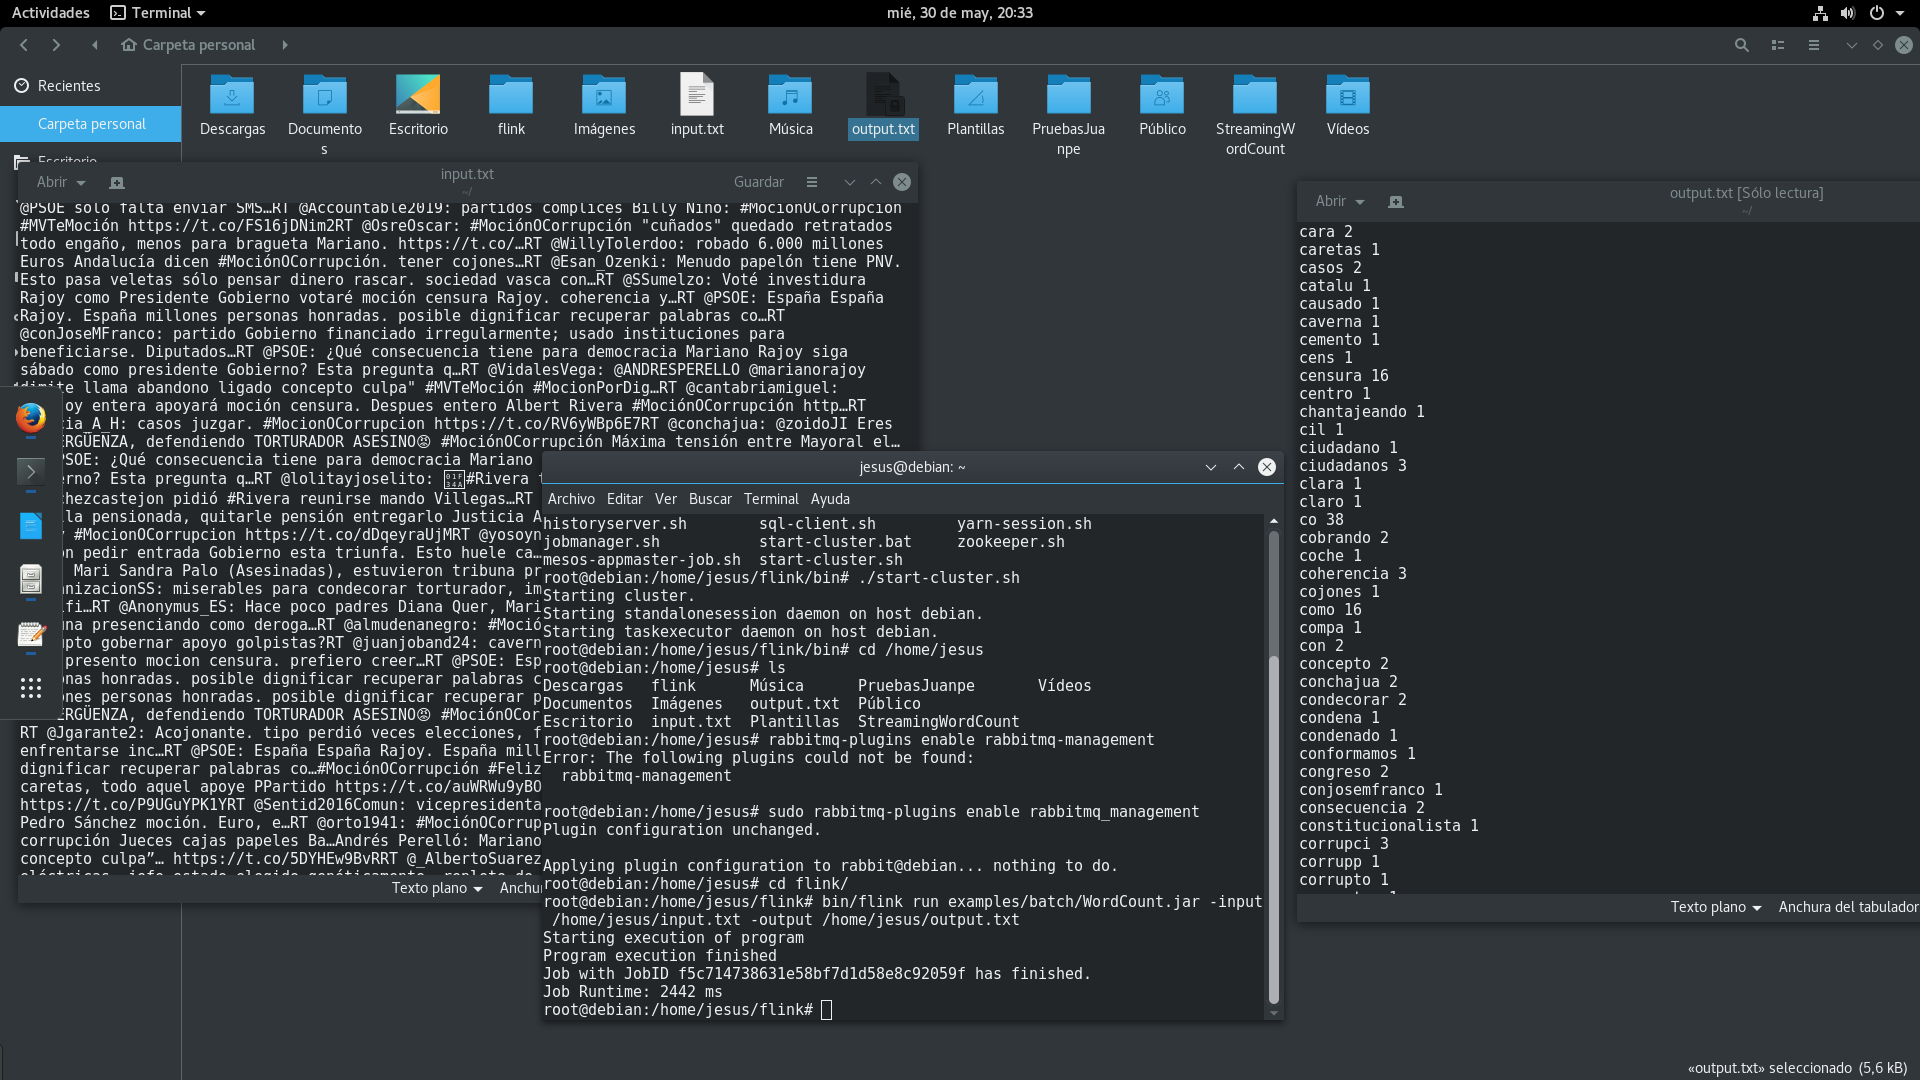
\includegraphics[scale=0.24]{18.png}
\end{center}

\section{Problemas encontrados}
El principal problema que nos encontramos a la hora de comenzar con el trabajo fue que directamente, no funcionaba en nuestro portátiles, por lo que nos pusimos manos a la obra con una máquina virtual en lubuntu, donde intentamos instalar Apache Flink pero, a la hora de ejecutar el código de prueba, saltaban muchas excepciones que no sabíamos controlar.\\

Visto esto, decidimos probar con una máquina virtual en Debian, en donde la instalación fue como la seda y el programa de prueba funcionó al primer intento.\\

Debido a que no contábamos con mucho tiempo, decidimos usar el ejemplo como idea, de tal forma que podíamos hacer una aplicación que nos diera las palabras más publicadas en twitter por la población española.

\section{Mejoras futuras}
En cuanto a mejorar el proyecto, podríamos filtrar las palabras recolectadas y eliminar las preposiciones y artículos, debido a que se repiten demasiado y no serían ``claves'' a la hora de buscar una palabra determinada si estamos haciendo un sondeo real.\\

Otra mejora a tener en cuenta es utilizar ``jpype'' que permite llamar a clases java desde python, lo que haría mucho más sencillo el trabajo de nuestro proyecto.

\section{Referencias}
\begin{itemize}
	\item \url{https://flink.apache.org/}
	\item \url{https://www.rabbitmq.com/}
	\item \url{https://en.wikipedia.org/wiki/Apache_Flink}
	\item \url{https://en.wikipedia.org/wiki/RabbitMQ}
	\item \url{https://www.adictosaltrabajo.com/tutoriales/introduccion-}\\\url{a-apache-flink/}
	\item \url{https://data-flair.training/blogs/install-configure-}\\\url{apache-flink-ubuntu/}
\end{itemize}



\end{document}